\documentclass[a4paper,12pt]{article}
\usepackage{amsmath}
\usepackage{amsfonts}
\usepackage{textcomp}
\usepackage{amssymb}
\usepackage{graphicx}
\usepackage{fancyhdr}
\usepackage[spanish]{babel}
\usepackage[utf8]{inputenc}
\usepackage{array}
\usepackage[usenames,dvipsnames,svgnames,table]{xcolor}
\usepackage{multirow}


\definecolor{niceblue}{RGB}{60,110,190}

\usepackage{vmargin}
\setpapersize{A4}
\setmarginsrb{2.5cm}{1.5cm}{2.5cm}{2.5cm}
{1cm}{0cm}%
{1cm}{1cm}

\begin{document}

\begin{tabular}{ >{\centering\arraybackslash}m{4cm} >{\arraybackslash}m{8cm}}
\fbox{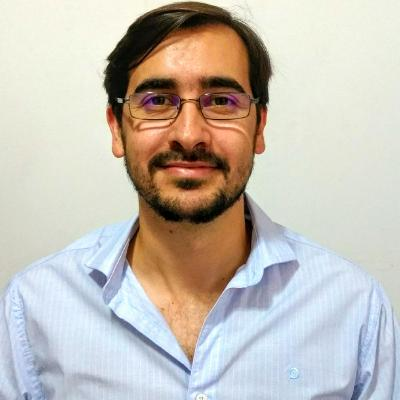
\includegraphics[width=25mm]{rodrigo}} & {\huge Dr. Rodrigo Baravalle} {\bf \em \color{CornflowerBlue} Postdoc (CONICET)}\\
\end{tabular}

\vspace{1cm}
\begin{tabular}{ll}
\bf{\color{Gray} Address} & Ocampo y Esmeralda, S2000EZP.\\
\bf{\color{Gray}Insitution} & CIFASIS, CONICET.\\
\bf{\color{Gray}City} & Rosario, Argentina\\
\bf{\color{Gray}Telephone} & +54 341 4815569\\
\bf{\color{Gray}Date of Birth}  & 20 April 1985\\
\bf{\color{Gray}Place of Birth}  & Rosario, Santa Fe, Argentina\\
\bf{\color{Gray}Marital Status}  & Single\\
\bf{\color{Gray}E-Mail} &baravalle@cifasis-conicet.gov.ar\\
\end{tabular}
\vspace{1cm}

\section*{\color{niceblue} About \rule{14cm}{2.2pt}}

\begin{small}
\noindent
I hold a PostDoc scolarship at the National Scientific and Technical Research Council (CONICET), Argentina. I defended my PhD thesis on March 2016 on the topic of Photo-realistic material modeling and simulation.
My foremost academic interests are Computer Graphics - Procedural Modeling - Texture Synthesis - Realistic Rendering - Volumetric Models - GPGPU - shading languages and Fractals. 
In addition, I am keen on reading about astronomy, physics and philosophy. Also, I eventually play chess.
\end{small}


\section*{\color{niceblue} Education \rule{12.8cm}{2.2pt}}

\begin{tabular}{lcp{9 cm}}
		\bf{2016} & & {\bf PhD in Informatics} (Photo-realistic material modeling and simulation). Facultad de Ciencias Exactas, Ingenier\'ia y Agrimensura - Universidad Nacional de Rosario. \\
		\bf{2010} & & {\bf Licenciateship in Computer Science}. Facultad de Ciencias Exactas, Ingenier\'ia y Agrimensura - Universidad Nacional de Rosario. Academic Average: 9.4 ``Distinguished''.\\
\end{tabular}

\newpage

\section*{\color{niceblue} Publications \rule{12.3cm}{2.2pt}}

\subsection*{\color{niceblue} Journals}

\begin{itemize}
\item {\bf Realistic Modeling of Porous Materials}. Rodrigo Baravalle, Leonardo Scandolo, Claudio Delrieux, Cristian García Bauza and Elmar Eisemann. In {\it Computer Animation \& Virtual Worlds}, 2016. doi:10.1002/cav.1719.
\item {\bf Procedural Bread Making}. Rodrigo Baravalle, Gustavo Patow and Claudio Delrieux. In {\it Computers \& Graphics}. {\bf 50}(2015):13-24. doi:10.1016/j.cag.2015.05.003.
\item {\bf Multifractal Characterisation and Classification of Bread Crumb Digital Images}. Rodrigo Baravalle, Claudio Delrieux and Juan Carlos Gómez. In {\it EURASIP Journal on Image and Video Processing}. {\bf 2015}:9. April 2015. doi:10.1186/s13640-015-0063-8.
\item {\bf Modeling for Photo-realistic Bread Rendering}. Rodrigo Baravalle, Leonardo Scandolo, Claudio Delrieux and Cristian García Bauza. In {\it Mecánica Computacional} ({\bf 33})26:1695-1709. Bariloche, Argentina. September 2014.
\item {\bf Bread Crumb Classification Using Fractal and Multifractal Features}. Rodrigo Baravalle, Claudio Delrieux and Juan Carlos G\'omez. In {\it Mecánica Computacional} ({\bf 31})17:3013-3025. Salta, Argentina. November 2012.
\end{itemize}

\subsection*{\color{niceblue} Technical Reports}
\begin{itemize}
\item {\bf 3D Mapping of Indoor Environments with a Time of Flight Camera}. Rodrigo Baravalle and Amaury N\`egre. E-MOTION (INRIA Grenoble Rh\^one-Alpes / LIG Laboratoire d'Informatique de Grenoble) Number: RT0406. Grenoble, France, February 2011.
\end{itemize}

\subsection*{\color{niceblue} Conferences}
\begin{itemize}
\item {\bf Experiencies with Cython and PyOpenCL}. In {\it Proceedings of the Second Conference of Python in Science}, SciPyConAr. Puerto Madryn, Argentina. October 2014.
\item {\bf Imfractal: fractal dimentions with Python}.  In {\it Proceedings of the First Conference of Python in Science}, SciPyConAr. Puerto Madryn, Argentina. May 2013.
\item {\bf Bread samples classification using fractal features}. Rodrigo Baravalle, Claudio Delrieux and Juan Carlos G\'omez. In {\it Proceedings of the V School in Science of Images}, ECIMAG. Santa Fe, Argentina, July 2012.
\item {\bf Procedimental Synthesis od Materials: results in bread modeling and cooked materials}. Rodrigo Baravalle, Claudio Delrieux and Juan Carlos G\'omez. In {\it Proceedings of the XIV Workshop of Researchers in Computer Science }, WICC. Posadas, Argentina, April 2012.
\item {\bf Texture Synthesis using Particle Systems}. Rodrigo Baravalle, Claudio Delrieux and Juan Carlos G\'omez. In {\it Proceedings of the Fourth School in Science of Images}, ECIMAG. Buenos Aires, Argentina, August 2011.
\item {\bf Procedimental generation of content in the development of video games}. Rodrigo Baravalle, Claudio Delrieux and Cristian Garc\'ia Bauza. In {\it Proceedings of the First argentine Workshop on video games}, WAVi. Buenos Aires, Argentina, December 2010.
\item {\bf A GPU Framework for Representing and Modeling Materials in Real Time }. Rodrigo Baravalle, Claudio Delrieux and Cristian Garc\'ia Bauza. In {\it Proceedings of the third School in Science of Images}, ECIMAG. Bahía Blanca, Argentina, July 2010.
\end{itemize}


\subsection*{\color{niceblue} Thesis}
\begin{itemize}
\item {\bf Photo-realistic material modeling and simulation}. Rodrigo Baravalle, Claudio Delrieux and Juan Carlos Gómez. Facultad de Ciencias Exactas, Ingeniería y Agrimensura, Universidad Nacional de Rosario, Argentina, March $28^{th}$, 2016.
\item {\bf A GPU Framework for Representing and Modeling Materials in Real Time}. Rodrigo Baravalle, Claudio Delrieux and Cristian García Bauza. Facultad de Ciencias Exactas, Ingeniería y Agrimensura, Universidad Nacional de Rosario, Argentina, August $10^{th}$, 2010.
\end{itemize}


\section*{\color{niceblue} Courses Given \rule{11.8cm}{2.2pt}}
\begin{itemize}
\item {\bf Introduction to Computer Graphics} at the Computer Science Department at UNR (Rosario, Argentina. November 2014).
\end{itemize}

\section*{\color{niceblue} Teaching Experience \rule{10cm}{2.2pt}}

Teacher assistant at the Computer Science Department at UNR (Rosario, Argentina) on different courses:
\begin{itemize}
\item Data Structures and Algorithms I. March - August 2012.
\item Computer Architectures. September 2012 - February 2013.
\end{itemize}

\section*{\color{niceblue} Work Experience \rule{11cm}{2.2pt}}

\begin{itemize}
\item {\bf Research Internship} at {\em IROBOT}, Pasadena, USA. Room Segmentation for robot vacuum cleaners. September 2015 - December 2015.
\item {\bf Research Internship} at {\em E-MOTION, Inria}, Grenoble, France. 3D Reconstruction from a Time-of-Flight Camera. September 2010 - February 2011.
\item {\bf Programmer} at {\em E-ducativa}, Rosario, Argentina. Perl + Javascript in web development. September 2008 - August 2010.
\item {\bf Programmer} at {\em UNR Campus Virtual}, Rosario, Argentina. PHP in web development. April - July 2008.
\end{itemize}

\section*{\color{niceblue} Grade Thesis Advised \rule{9.6cm}{2.2pt}}
\begin{itemize}
\item {\bf Reconstrucción 3D densa sobre sistemas de SLAM basados en visión estéreo}. Ariel D'Alessandro, Co-Advisor. Universidad Nacional de Rosario, Argentina, {\it In Progress}.
\end{itemize}

\section*{\color{niceblue} Grade Thesis Evaluator \rule{9.1cm}{2.2pt}}
\begin{itemize}
\item {\bf Aprendizaje Multiclase de Videoimágenes deportivas con Arquitecturas Profundas}. Martín Escarrá. Universidad Nacional de Rosario, Argentina.
\end{itemize}



\section*{\color{niceblue} Post Graduate Semester Courses Attended \rule{3.5cm}{2.2pt}}
\begin{itemize}
\item {\bf Digital Image Processing}, Universidad Nacional de Rosario, Argentina. Given by Dr. Guillermo Kaufmann, Phd. Grade: 9 (Nine).
\item {\bf Computer Graphics}, UBA, Buenos Aires, Argentina. Given by Dr. Claudio Delrieux, Phd. (UNS, Argentina). Grade: 10 (Ten).
\item {\bf Fractal Models and Chaotic Systems in Computational Physics and Natural Sciences}, DIEC, UNS, Bah\'ia Blanca, Argentina. Given by Dr. Claudio Delrieux, Phd. (UNS, Argentina). Grade: 10 (Ten).
\end{itemize}


\section*{\color{niceblue} Disertations \rule{12.5cm}{2.2pt}}
\begin{itemize}
\item {\bf Photo-realistic material modeling and simulation}, PhD Thesis. March 2016, Rosario, Argentina.
\item {\bf Modeling for Photo-realistic Bread Rendering}, at the $21^{th}$ ENIEF. September 2014, Bariloche, Argentina.
\item {\bf Bread Crumb Classification Using Fractal and Multifractal Features}, at the $10^{th}$ MECOM. November 2012, Salta, Argentina.
\item {\bf Texture Synthesis using Particle Systems}, at the $4^{th}$ ECImag. August 2011, Buenos Aires, Argentina.
\item {\bf A Framework in GPU for Representing and Modeling Materials in Real Time}, Master Thesis. August 2010, Rosario, Argentina.
\item {\bf A Framework in GPU for Representing and Modeling Materials in Real Time}, at the $3^{rd}$ ECImag. July 2010, Bahía Blanca, Argentina.
\end{itemize}


\section*{\color{niceblue} Courses Attended \rule{10cm}{2.2pt}}
\begin{itemize}
\item {\bf Fractal and Multifractal Analysis of Complex Systems}, at the $2^{a}$ ECIMAG 2012, organized by UNS, Universidad Nacional del Sur. Given by Dra. Tatijana Stosic, Phd (Universidade Federal Rural de Pernambuco, Recife, PE, Brazil).
\item {\bf Parallel Programming in GPU}, at the $4^{th}$ ECImag 2011, organized by ITBA, Instituto Tecnol\'ogico de Buenos Aires. Given by Dr. Juan Pablo D'amato, Phd (Universidad Nacional del Centro, Argentina).
\item {\bf Visualization of Algebraic Surfaces}, at the $4^{th}$ ECImag 2011, organized by ITBA, Instituto Tecnol\'ogico de Buenos Aires, given by Dr. Andreas Matt, Phd (Mathematisches Forschungsinstitut Oberwolfach, Germany). Grade: 8 (Eight).
\item {\bf A Practical Introduction to 3D Computer Vision}, at the $3^{rd}$ ECImag 2010, organized by DIEC, Universidad Nacional del Sur. given by Dr. Radim S\'ara, Phd (Politechnic Institute of Prague, Czech Republic).
\item {\bf Procedural Modeling}, at the $3^{rd}$ ECImag 2010, organized by DIEC, Universidad Nacional del Sur. Given by Dr. Gustavo Patow, Phd. (Applied Mathematics Dept. University of Girona, Spain).
\item {\bf Patterns in Game Development}, at the $2{nd}$ ECImag 2009, organized by the Institute PLADEMA. Facultad de Ciencias Exactas. Universidad Nacional del Centro. Given by Dr. Federico Balaguer, Phd. (LIFIA, Universidad Nacional de La Plata, La Plata, Argentina).
\item {\bf Fractals: applications to image processing and computer graphics}, at the $2{nd}$ ECImag 2009, organized by the Institute PLADEMA. Facultad de Ciencias Exactas. Universidad Nacional del Centro. Given by Dr. Claudio Delrieux, Phd. (Universidad Nacional del Sur, Bah\'ia Blanca).
\item {\bf Image Processing}, at the $14{th}$ RIO 2007, organized by the Department of Computer Science, UNRC. Given by Dr. Rafael Lins, Phd. (Federal University of Pernambuco, Brazil). Grade: 10 (Ten).
\item {\bf Category Theory}, at the $14{th}$ RIO 2007, organized by the Department of Computer Science, UNRC. Given by Dr. Mat\'ias Menni, Phd. (LIFIA,UNLP,Argentina).
\item {\bf Lectures of Introduction to Quantum Computation}, organized by the Computer Science Department, FCEIA, UNR. Given by Alejandro Diaz-Caro, student of Computer Science.
\end{itemize}

\section*{\color{niceblue} Scholarships Granted \rule{10cm}{2.2pt}}

\begin{itemize}
\item September 2015 - December 2015, Internship at IROBOT, Pasadena, USA. Topic: Room Segmentation for robot vacumm cleaners.
\item April 2014 - April 2016, Type II Postgraduate scholarship, CONICET, Argentine.
\item April 2011 - April 2014, Type I Postgraduate scholarship, CONICET, Argentine.
\item September 2010 - February 2011, Internship at INRIA (Institut national de recherche en informatique et automatique), eMotion team, Grenoble, France. Topic: 3D Mapping.
\item January - February 2008, IMPA (Institute for Pure and Applied Mathematics), R\'io de Janeiro, Brasil - Summer course on Computer Graphics.

\end{itemize}

\section*{\color{niceblue} Participation in Acredited Projects \rule{5.8cm}{2.2pt}}

\begin{itemize}
\item January 2013 - December 2016, {\bf Multimedia signal processing - Applications to multimodal speech processing, automatic verification of handwritten signatures and non-linear system identification}. Project id: ING427. Acredited by Universidad Nacional de Rosario, Argentine.
\item January 2011 - December 2012, {\bf Digital image processing - Applications to audio-visual speech processing, digital watermarking, automatic recognition of handwritten signatures and recognition of vegetal species from leaf vein images}. Project id: ING355. Acredited by Universidad Nacional de Rosario, Argentine.

\end{itemize}



\section*{\color{niceblue} Scientific Meetings \rule{10.7cm}{2.2pt}}
\begin{small}
\begin{itemize}
\item $2^{nd}$ ScipyConAr. Argentine School of Scientific Computing with Python, October 2014.
\item $21^{th}$ ENIEF,  Congress on Numerical Methods and its Applications, September 2014.
\item $1^{st}$ ScipyConAr. Argentine School of Scientific Computing with Python, May 2013.
\item $10^{th}$ MECOM. Argentine Congress of Computational Mechanics, September 2012.
\item $5^{th}$ ECImag. Workshop on Image Science, July 2012.
\item $4^{th}$ ECImag. Workshop on Image Science, August 2011.
\item $1^{st}$ PEAGPGPU. Workshop on GPGPU computing for Scientific Applications, May 2011.
\item $3^{rd}$ ECImag. Workshop on Image Science, July 2010.
\item $7^{th}$ JCC, Rosario, Argentina, October 2009.
\item $2^{nd}$ ECImag. Workshop on Image Science, September 2009.
\item $6^{th}$ JCC, Rosario, Argentina, October 2008.
\item $5^{th}$ JCC, Rosario, Argentina, October 2007.
\item STIC-AmSud, 3rd French-South American scientific cooperation programme on sciences and technologies of informatics and communications, Montevideo, Uruguay. November 2007.
\item $14^{th}$ RIO, R\'io Cuarto, Argentina, February 2007.
\item $2^{nd}$ JAI, Rosario, Argentina, December 2006.
\item $4^{th}$ JCC, Rosario, Argentina, October 2006.
\item $3^{rd}$ JCC, Rosario, Argentina, December 2005.
\end{itemize}
\end{small}


\section*{\color{niceblue} Languages \rule{13.2cm}{2.2pt}}

\begin{small}
\begin{description}
	\item[Spanish:] Native language.
	\item[English:] First Certificate In English (FCE) (Level B2), by University of Cambridge, ESOL. Certificate Number: 0026091410. February 2010.
	\item[French:] DELF B2 Certificate (Level B2), by Alliance Fran\c{c}aise. Certificate number: 054041-201311T-2234032. April 2014.
	\item[Portuguese:] Can Read.
\end{description}
\end{small}

\section*{\color{niceblue} References \rule{13cm}{2.2pt}}

\begin{itemize}
	\item {\bf Dr. Gustavo Patow}, PhD. Head of the Geometry and Graphics Group (GGG), Girona, Spain.\\E-mail: dagush@imae.udg.edu \\
	\item {\bf Dr. Mario Munich}, PhD. SVP Technology, IROBOT, Pasadena, USA.\\E-mail: mmunich@irobot.com. \\
	\item {\bf Dr. Alexander Kleiner}, PhD. Senior Principal Robotics Scientist. IROBOT, Pasadena, USA.\\E-mail: alexander.kleiner@gmail.com. \\
	\item {\bf Dr. Claudio Delrieux}, PhD. Head of the Department of Electrical Engineering and Computers, Universidad Nacional del Sur, Argentina.\\E-mail: cad@uns.edu.ar\\
	\item {\bf Dr. Juan Carlos G\'omez}, PhD. Head of the Laboratory of Dynamical Systems and Information Processing, Universidad Nacional de Rosario, Argentina.\\E-mail: jcgomez@fceia.unr.edu.ar\\
	\item {\bf MSc. Amaury Nègre}, Research Engineer at E-MOTION Group, Inria, Grenoble, France.\\E-mail: amaury.negre@inrialpes.fr. \\
\end{itemize}

\end{document}




